%
% $Author: Abishek $
% $Date: 06.01.2025 $
% $Path: ML24-02-Gait-Pattern-Recognition\report\Contents\en$
% $Version: 1.0 $
% $Reviewed by: Abishek $
%
% !TeX encoding = utf8
% !TeX root = Rename
% !TeX TXS-program:bibliography = txs:///bibtex
%
%%%%%%
\chapter{Knowledge Discovery in Databases (KDD)}

The Knowledge Discovery in Databases (KDD) process is an essential methodology for extracting meaningful insights and patterns from data. This chapter discusses the major components involved in the KDD pipeline, focusing on data selection, processing, and augmentation, particularly in the context of our project involving gait pattern recognition. The following sections provide a comprehensive overview of each stage.

\subsection{Origin}
The dataset is stored in a CSV file and hosted on a Git repository which is publicly available\url{https://github.com/Zhang-Wenwen/GaitMotion}. The data is accessed programmatically using Python (Pandas, NumPy) for preprocessing and analysis.The origin of the data is critical for understanding the context and reliability of the dataset. In this project, the dataset is used to train a Convolutional Neural Network (CNN) machine learning model in Python to classify user gait as normal or Parkinsonian. The data used in this project comes from the GaitMotion dataset, which was specifically designed for gait analysis. This dataset was collected using wearable inertial measurement units (IMUs), such as accelerometers and gyroscopes, placed on participants to capture motion data along six axes (X, Y, Z for both sensors).

Participants were instructed to simulate both normal and Parkinsonian gaits, and the sensors were positioned on their feet, which provide more accurate and direct measurements of foot movement and ground contact compared to placements on the shank or thigh. To ensure the reliability and precision of the dataset, data collection was conducted in controlled environments and synchronized with validated tools like the GaitRite system\cite{Webster:2005}. These measures make the dataset suitable for training machine learning models aimed at accurately detecting gait patterns.\cite*{ZhangWenwen:2022}

\subsection{Features}

Features are the variables extracted and used to classify gait patterns as normal or Parkinsonian. In this project, data is collected from sensors placed on a single leg, focusing on detailed motion characteristics from that leg. The key features selected for this project include:

\begin{itemize}
	\item \textbf{Raw Sensor Data}:
	\begin{itemize}
		\item Accelerometer data: X, Y, Z axes.
		\item Gyroscope data: X, Y, Z axes.
	\end{itemize}
	These raw measurements from a single leg capture motion, orientation, and rotational changes, serving as the basis for further feature engineering.
	
	\item \textbf{Stride Length}:
	The distance covered by one stride, derived from accelerometer and gyroscope data, is a key feature to identify differences in walking patterns.
	
	\item \textbf{Stride Time}:
	The duration of a single stride, calculated using temporal patterns in the data, is an important indicator for detecting gait irregularities.
	
	\item \textbf{Stride Velocity}:
	The speed at which a stride is completed, computed using stride length and stride time, provides insights into the overall walking pace.
	
	\item \textbf{Step Variability}:
	Measures fluctuations in stride length or stride time, offering clues about irregular gait patterns, which are more pronounced in Parkinsonian gaits.
	
	\item \textbf{Angular Velocity}:
	Derived from gyroscope data, it measures rotational movement of the leg, crucial for detecting turning movements or balance issues.
	
	\item \textbf{Magnitude Features}:
	Magnitude of acceleration (\( \sqrt{x^2 + y^2 + z^2} \)) and angular velocity captures the intensity of leg motion during walking.
	

\end{itemize}

By focusing on data from a single leg, this approach minimizes complexity while retaining the ability to capture meaningful gait dynamics. The derived features, combined with raw sensor data, enable the CNN model to effectively differentiate between normal and Parkinsonian gaits. \cite{ZhangWenwen:2022}

\subsection{Data Types}

The dataset used in this project includes various types of data derived from IMU sensor readings, which are combined to classify gait patterns as normal or Parkinsonian. The types of data in the dataset are as follows:

\begin{itemize}
	\item \textbf{Numerical Data}:
	\begin{itemize}
		\item The dataset primarily consists of numerical features calculated from raw sensor readings, including:
		\begin{itemize}
			\item Step length, stride length, and stride velocity.
			\item Step time, stride time, stance time, and swing time.
			\item Support base, support time, and related variables capturing gait characteristics.
			\item Measurements like foot length, foot width, and other spatial metrics.
		\end{itemize}
		\item These features are represented as continuous numerical values and form the foundation for machine learning analysis.
	\end{itemize}
	
	\item \textbf{Categorical Data}:
	\begin{itemize}
		\item Each segment of the dataset is labeled as either \textbf{0} (normal gait) or \textbf{1} (Parkinsonian gait), indicating the classification target.
	\end{itemize}
	
	\item \textbf{Temporal Data}:
	\begin{itemize}
		\item The data captures time-dependent features such as step time, stride time, and swing time, which reflect variations in gait over time.
	\end{itemize}
\end{itemize}

By combining numerical, categorical, and temporal data, the dataset provides a comprehensive representation of gait dynamics, allowing the CNN model to effectively learn the differences between normal and Parkinsonian gaits.\cite{ZhangWenwen:2022}

\subsection{Quality}

The quality of the dataset is critical for ensuring accurate and reliable results in gait analysis. The GaitMotion dataset was meticulously collected to address limitations commonly found in gait analysis datasets. Key aspects of data quality include:

\begin{itemize}
	\item \textbf{Ground-Truth Synchronization:}
	The dataset is synchronized with the GaitRite system, which ensures accurate labeling of gait events such as heel strikes and toe-offs. This provides reliable ground-truth data for step segmentation and gait parameter estimation.
	
	\item \textbf{Controlled Data Collection:}
	Data was recorded under controlled environments to minimize noise and variability. Participants performed tasks on a GaitRite carpet, ensuring consistent conditions across trials.
	
	\item \textbf{Minimization of Errors:}
	To reduce missing or overcounting steps, data was collected with high-precision IMUs placed on participants’ feet. Calibration processes, such as stationary periods before and after trials, further enhanced data quality by addressing mean value drifts.
	
	\item \textbf{Balanced Dataset:}
	The dataset includes diverse walking patterns (normal, Parkinsonian, and stroke gaits) to ensure comprehensive coverage of gait variations. This diversity supports the development of robust machine learning models.\cite{ZhangWenwen:2022}
\end{itemize}

These measures ensure the GaitMotion dataset's reliability and make it a valuable resource for training and testing machine learning models for gait analysis.

\subsection{Quantity}

The quantity of data directly impacts the robustness of machine learning models. The GaitMotion dataset includes:

\begin{itemize}
	\item \textbf{Data Volume:}
	The dataset contains recordings from 10 participants performing three different walking patterns: normal, Parkinsonian, and stroke. Each participant performed six trials per walking pattern, resulting in a total of 180 trials.
	
	\item \textbf{Data Diversity:}
	With over 1,000 strides recorded across all participants and walking patterns, the dataset provides sufficient data points for training, validation, and testing.
	
	\item \textbf{Temporal and Spatial Coverage:}
	Each trial captures detailed temporal and spatial parameters, including step segmentation, stride length, stride time, stance time, and swing time.\cite{ZhangWenwen:2022}
\end{itemize}

The extensive quantity of high-quality data ensures that machine learning models trained on this dataset can generalize well and produce accurate results in real-world applications.

\subsection{ Fairness/Bias}

Ensuring fairness and reducing bias in the dataset is a critical aspect of this project. The following measures were implemented:

\begin{itemize}
	\item \textbf{Balanced Dataset:}
	The dataset includes an equal number of trials for normal and Parkinsonian gaits, ensuring the machine learning model does not favor one class over the other.
	
	\item \textbf{Consistent Data Collection:}
	All data was collected in controlled environments using the same sensor placements and standardized procedures to avoid variations caused by experimental conditions.
	
	\item \textbf{Bias Detection and Mitigation:}
	Any errors or outliers were removed from the dataset to improve data quality. For example, the first and last strides of each trial were excluded to avoid inaccuracies from starting or stopping movements.
	
\end{itemize}

These steps were carefully followed to minimize bias and create a fair dataset for training and testing the machine learning model.



\section{Data Processing}

Once the data is selected, it undergoes several preprocessing steps to prepare it for model training. The primary objectives of data processing include cleaning, normalization, and feature extraction.

\subsection{One Database}
All collected data was consolidated into a single database to maintain consistency and simplify the modeling process. The dataset originally included data for both left and right legs across 10 participants performing normal, Parkinsonian, and stroke gaits. For this project, only the data from the right leg was retained to reduce redundancy and focus on key features.

Data from normal and Parkinsonian gaits were combined into a single CSV file, with labels indicating the gait type: 0 for normal and 1 for Parkinsonian. Features that were only relevant for dual-leg analysis were excluded, ensuring the final database contained only meaningful and necessary information. This consolidation into a single CSV file ensures efficient preprocessing, querying, and analysis during the development of the machine learning model.

\subsection{Properties}

The properties of the data were carefully studied to ensure it is ready for machine learning. The key aspects examined include:

\begin{itemize}
	\item \textbf{Distribution:}
	The range and spread of features like stride length, stride time, and stride velocity were checked to ensure the data covers both normal and Parkinsonian gaits properly. Any imbalances were noted and addressed.
	
	\item \textbf{Relationships:}
	The connections between features, such as how stride time relates to stride velocity, were analyzed. This helped identify which features provide the most useful information for classifying gaits.
	
	\item \textbf{Stationarity:}
	Time-related features like step time and stride time were checked to see if their values stayed consistent over time. Adjustments like normalization were applied if needed.
	
	\item \textbf{Outliers:}
	Any unusual data points, like extremely high or low stride lengths, were identified and removed to ensure they don’t affect the model’s performance.
\end{itemize}

These steps ensure the data is clean, balanced, and ready for building an accurate machine learning model.


\subsection{Outliers}

Outliers in the dataset were carefully identified and addressed to maintain the accuracy and reliability of the machine learning model. These outliers were primarily observed in features such as stride velocity, which can significantly affect model performance.

\paragraph{Detection}
\begin{itemize}
	\item Outliers were detected by analyzing the distribution of stride velocity in relation to stride length. A scatterplot (shown below) was used to visualize the data and identify extreme values.
	\item A threshold was set for stride velocity, and values exceeding \textbf{150 cm/s} were flagged as outliers, as they were considered unrealistic based on domain knowledge.\cite{perry2010gait}
\end{itemize}

\paragraph{Handling}
\begin{itemize}
	\item Data points with stride velocity values greater than \textbf{150 cm/s} were reviewed and handled as follows:
	\begin{itemize}
		\item Extreme outliers caused by sensor noise or data collection errors were removed.
		\item Data points that slightly exceeded the threshold were replaced with the median stride velocity value for similar stride lengths.
	\end{itemize}
\end{itemize}

\paragraph{Visualization}
The scatterplot  \ref{fig:outlier} illustrates the relationship between stride length and stride velocity, with outliers highlighted above the threshold:

	\begin{figure}[h]
	\centering
	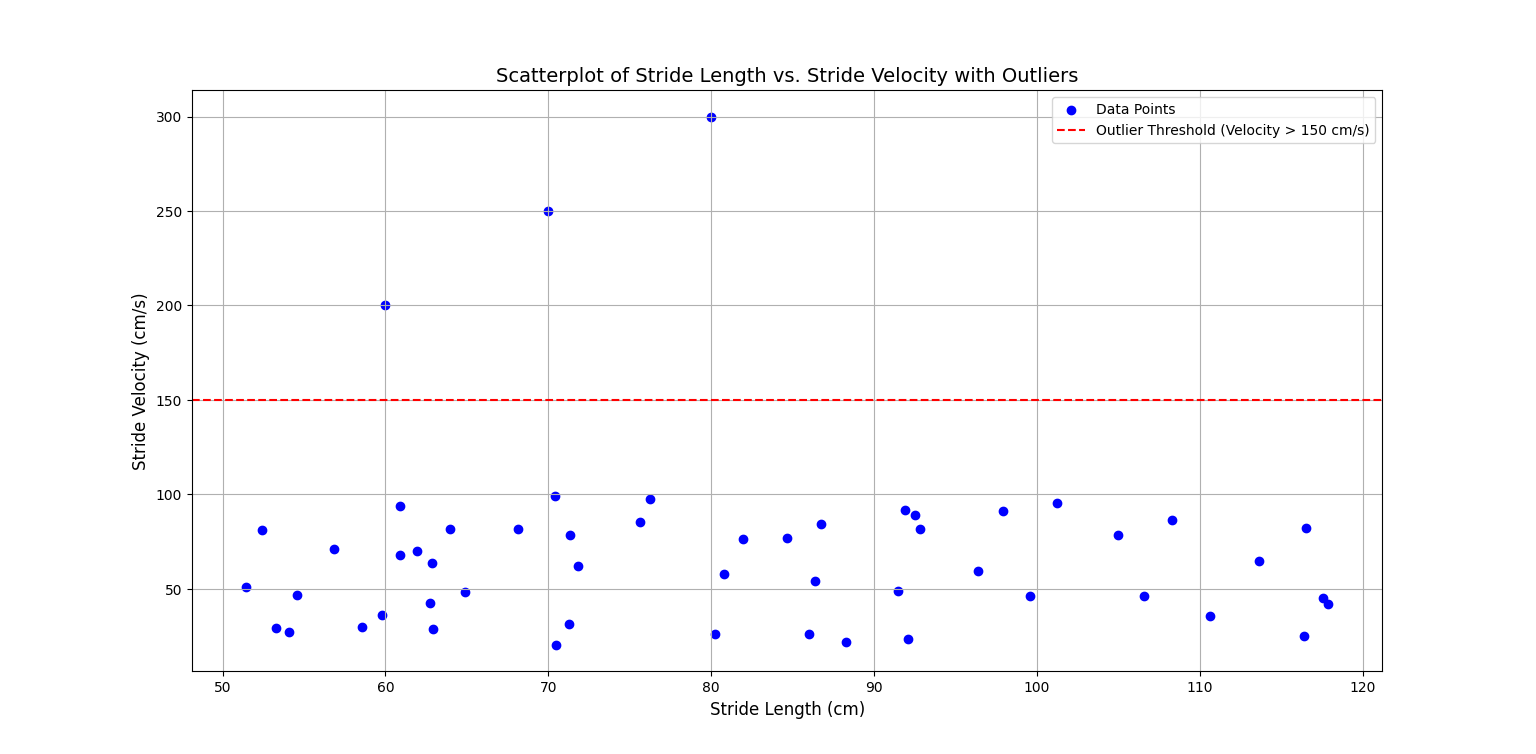
\includegraphics[width=0.7\textwidth]{Images/Outlier}
	\caption {Scatterplot of Stride Length vs. Stride Velocity with Outliers. Data points above the red dashed line (velocity > 150 cm/s) represent outliers.}
	\label{fig:outlier}
\end{figure}



By systematically identifying and addressing outliers, the dataset was refined to remove extreme values that could distort patterns. This process ensures that the model is trained on high-quality data, improving its ability to classify normal and Parkinsonian gaits accurately.


\subsection{Anomalies}

Anomalies are unusual patterns in the data that could skew results. In this project, anomalies were identified by analyzing features like stride length and velocity. Values outside typical ranges, such as stride lengths below 10 cm or velocities above 200 cm/s, were flagged. 

To address these anomalies:
\begin{itemize}
	\item Minor anomalies were corrected by replacing them with median values.
	\item Extreme anomalies caused by sensor errors were removed entirely.
\end{itemize}

\subsection{Augmentation}

Data augmentation was applied to improve the dataset's diversity and model robustness:
\begin{itemize}
	\item \textbf{Synthetic Data Generation:} New data points were created by varying stride features within acceptable ranges.
	\item \textbf{Noise Addition:} Random noise was added to simulate real-world variations.
	\item \textbf{Temporal Augmentation:} Overlapping strides were used to create additional data points.
\end{itemize}

These techniques enriched the dataset and enhanced the model’s ability to generalize.

\section{Data Transformation}

Data transformation is a crucial step in preparing the dataset for machine learning analysis. This process involves consolidating, encoding and optimizing the data for efficient model training and evaluation.

\subsection{Data Consolidation}
\begin{itemize}
	\item Data from normal and Parkinsonian gaits were merged into a single CSV file to maintain consistency and ease of access.
	\item Labels were assigned to indicate gait types:
	\begin{itemize}
		\item \textbf{0} - Normal gait
		\item \textbf{1} - Parkinsonian gait
	\end{itemize}
	\item Features relevant only to dual-leg analysis were excluded to eliminate redundancy and retain essential gait characteristics.
\end{itemize}

\subsection{Feature Selection and Engineering}
\begin{itemize}
	\item Selected features focused on single-leg motion to simplify the dataset while preserving meaningful information.
	\item Irrelevant or highly correlated features were removed to enhance model interpretability and performance.
\end{itemize}

\subsection{Data Storage Optimization}
\begin{itemize}
	\item The transformed dataset was stored in a structured CSV format, ensuring efficient preprocessing, querying and analysis during the development of the machine learning model.
	\item The final dataset was structured for seamless integration with Python-based analysis tools like Pandas and NumPy.
\end{itemize}

\section{Data Mining}

This section details the application of data mining in our project, focusing on hyperparameters, input data, training, interpretation and output.

\subsection{Application in our Project}
In our project, data mining is applied to distinguish between normal and Parkinsonian gait patterns using a Convolutional Neural Network (CNN). The key steps include:
\begin{itemize}
	\item Preprocessing raw sensor data using Kalman Filtering to smooth out noise.
	\item Extracting relevant features from stride data.
	\item Training a CNN model to classify gait patterns.
	\item Exporting the trained model for deployment on embedded systems.
	\item Visualizing predictions to evaluate performance.
\end{itemize}

\section{Hyperparameters}
The main hyperparameters used in our CNN model are:

\begin{itemize}
	\item \textbf{Learning Rate}: Adjusted dynamically to optimize convergence.
	\item \textbf{Batch Size}: Set to 32 to balance training speed and generalization.
	\item \textbf{Number of Epochs}: Set to 50, ensuring sufficient training iterations.
	\item \textbf{Kernel Size}: 3x3 filters used in convolutional layers for feature extraction.
	\item \textbf{Dropout Rate}: Applied to prevent overfitting, set at 0.3.
	\item \textbf{Activation Function}: ReLU used for hidden layers, Softmax for output classification.
\end{itemize}

\section{Input Data}

The input data consists of gait patterns stored in CSV files. The main datasets are:

\begin{itemize}
	\item \textbf{Normal Gait Dataset}: \FILE{normalpatterns.csv}
	\item \textbf{Parkinsonian Gait Dataset}: \FILE{parkinsonpatterns.csv}
\end{itemize}

Each dataset contains six-axis IMU sensor data (accelerometer and gyroscope readings) and extracted features such as stride length, stride time and angular velocity.

\section{Training Process}

The training pipeline follows these steps:

\begin{enumerate}
	\item \textbf{Data Loading}: The datasets are loaded using a custom \SHELL{loadData} function.
	\item \textbf{Preprocessing}: The Kalman Filter is applied to smooth sensor readings and remove noise.
	\item \textbf{Model Training}: A CNN model is created using TensorFlow and trained on the processed data.
	\item \textbf{Validation}: Model performance is evaluated using accuracy and loss metrics.
	\item \textbf{Export}: The trained model is converted to TensorFlow Lite format and saved as a file \FILE{.h} for embedded deployment.
\end{enumerate}

\section{Interpretation of Results}

To interpret model predictions, visualization techniques are employed:

\begin{itemize}
	\item \textbf{Prediction Visualization}: Model predictions are plotted against actual labels to assess accuracy.
	\item \textbf{Confusion Matrix}: Used to evaluate classification performance.
	\item \textbf{Feature Importance}: Analyzed to understand which gait parameters contribute most to classification.
\end{itemize}

\section{Output and Deployment}

The model achieved 82\% classification accuracy in distinguishing between normal and Parkinsonian gait patterns using single-leg gait features as shown in the figure ~\ref{fig:output}.

\begin{figure}[h]
	\centering
	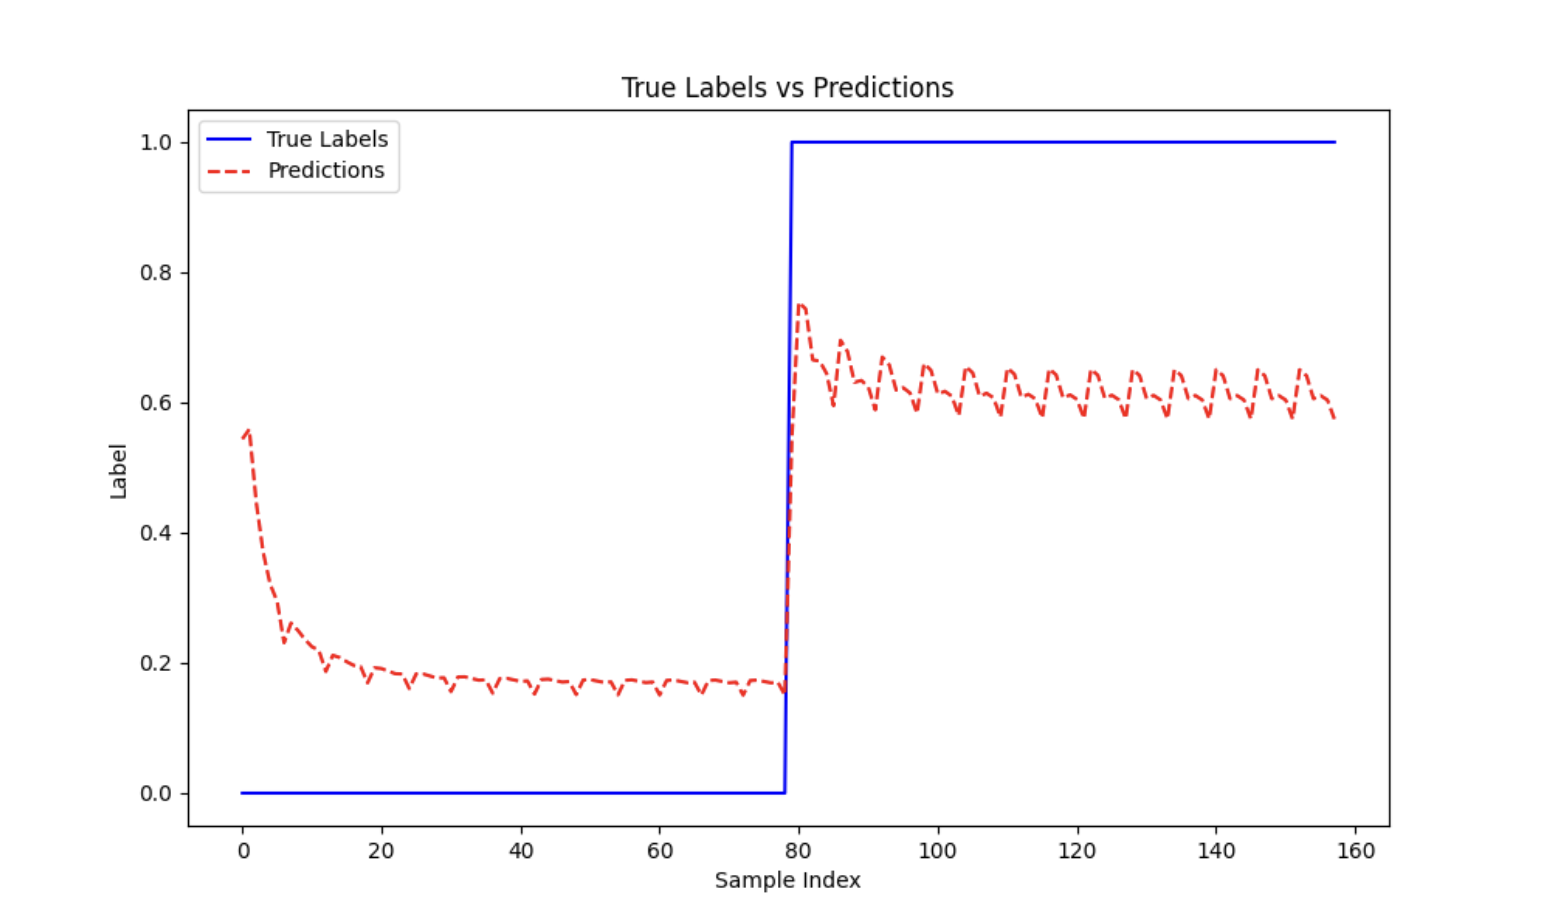
\includegraphics[width=0.7\textwidth]{Images/PredictionVisual}
	\caption {Output Model prediction}
	\label{fig:output}
\end{figure}

This structured approach ensures effective gait pattern recognition using data mining techniques.

\chapter{Documentation Developer}

\section{Idea}
The Parkinson Gait Pattern Recognition project aims to classify gait patterns as either normal or Parkinsonian using machine learning. The pipeline involves:
\begin{itemize}
	\item Loading gait datasets.
	\item Preprocessing data using a Kalman Filter.
	\item Training a Convolutional Neural Network (CNN).
	\item Exporting the trained model to TensorFlow Lite.
	\item Generating a \FILE{.h} file for Arduino integration.
	\item Visualizing predictions.
\end{itemize}

\section{Flow Chart of Each Step}

The flowchart in the figure ~\ref{fig:gait_pipeline_flowchart} provides a high-level overview of the key stages involved in the gait recognition pipeline, from data loading to model exportation and prediction visualization.

\begin{figure}[h]
	\centering
	\tikzset{
		startstop/.style = {rectangle, rounded corners, minimum width=3cm, minimum height=1cm, text centered, draw=black, fill=red!30},
		process/.style = {rectangle, minimum width=3cm, minimum height=1cm, text centered, draw=black, fill=blue!20},
		arrow/.style = {thick,->,>=stealth}
	}
	
	\begin{tikzpicture}[node distance=2cm]
		
		% Nodes
		\node (start) [startstop] {Start};
		\node (loadData) [process, below=of start] {Load Dataset (CSV)};
		\node (preprocess) [process, below=of loadData] {Apply Kalman Filter};
		\node (featureExtract) [process, below=of preprocess] {Extract Features};
		\node (trainModel) [process, below=of featureExtract] {Train CNN Model};
		\node (exportModel) [process, below=of trainModel] {Export to TFLite \& .h};
		\node (visualize) [process, below=of exportModel] {Visualize Predictions};
		\node (end) [startstop, below=of visualize] {End};
		
		% Arrows
		\draw [arrow] (start) -- (loadData);
		\draw [arrow] (loadData) -- (preprocess);
		\draw [arrow] (preprocess) -- (featureExtract);
		\draw [arrow] (featureExtract) -- (trainModel);
		\draw [arrow] (trainModel) -- (exportModel);
		\draw [arrow] (exportModel) -- (visualize);
		\draw [arrow] (visualize) -- (end);
		
	\end{tikzpicture}
	
	\caption{Flowchart of the gait pattern recognition pipeline}
	\label{fig:gait_pipeline_flowchart}
\end{figure}


\section{Notation}
Consistent and clear notation is used throughout the documentation. This includes naming
conventions for functions, variables and modules like:
\begin{itemize}
	\item X : Input dataset.
	\item Y : Output labels (0 = normal, 1 = Parkinsonian).
	\item KF(X) : Kalman Filter applied to input data.
	\item CNN(X) : Convolutional Neural Network model.
	\item TFL(X) : TensorFlow Lite model.
	\item H(X) : Model exported as a header file for Arduino.
\end{itemize}

\section{Completeness}
The project follows a structured pipeline ensuring completeness:
\begin{itemize}
	\item Data collection from CSV files.
	\item Preprocessing with Kalman Filtering.
	\item Feature extraction.
	\item CNN Model training and evaluation.
	\item Exporting to TensorFlow Lite and \FILE{.h} format for deployment.
	\item Visualization of predictions for performance validation.
\end{itemize}

\section{Machine Learning Pipeline}
\begin{enumerate}
	\item \textbf{Data Loading:} Reads CSV files (\FILE{normalpatterns.csv, parkinsonpatterns.csv}).
	\item \textbf{Preprocessing:} Applies Kalman Filter for noise reduction. \cite{Welch:1995}
	\item \textbf{Feature Extraction:} Reshapes data into CNN-compatible format.
	\item \textbf{Model Training:} CNN trained on processed data.
	\item \textbf{Model Exporting:} Converts trained model to TensorFlow Lite (\FILE{.tflite}).
	\item \textbf{Deployment Preparation:} Generates a \FILE{.h} file for Arduino.
\end{enumerate}

\section{Program}

\subsection{Readability}
\begin{itemize}
	\item Clear and structured code with meaningful variable and function names.
	\item Sufficient comments for better understanding.
\end{itemize}

\subsection{Structure/Modules}
The project is organized into separate modules:
\begin{itemize}
	\item \FILE{main.py} - Entry point for pipeline execution.
	\item \FILE{src/dataloader.py} - Loads gait data.
	\item \FILE{src/kalmanfilter.py} - Applies Kalman Filter.
	\item \FILE{src/cnnmodel.py} - Defines CNN model.
	\item \FILE{src/visualization.py} - Generates prediction visualizations.
	\item \FILE{src/tfliteexporter.py} - Converts model to TensorFlow Lite and exports to \FILE{.h}.
	\item \FILE{src/logger.py} - Logging setup.
	\item \FILE{src/config.py} - Stores default parameters.
\end{itemize}

\subsection{Parameter Handling}
Pipeline parameters are managed in \FILE{src/config.py}, including:
\begin{itemize}
	\item Number of epochs (\PYTHON{cnnEpochs}).
	\item Batch size (\PYTHON{cnnBatchSize}).
	\item Validation split (\PYTHON{cnnValidationSplit}).
\end{itemize}

\subsection{Error Handling}
\begin{itemize}
	\item Uses try-except blocks to catch errors.
	\item Logs errors using \PYTHON{logging.error()}.
\end{itemize}

\subsection{Message Handling}
\begin{itemize}
	\item Informational messages logged using \PYTHON{logging.info()}.
	\item Warnings and errors are logged separately.
\end{itemize}

\subsection{Naming Conventions}
\subsubsection{Folders}
\begin{itemize}
	\item \FILE{models/} - Stores exported model files.
	\item \FILE{src/} - Contains all Python modules.
	\item \FILE{data/} - Stores dataset files.
\end{itemize}

\subsubsection{Files}
\begin{itemize}
	\item \FILE{main.py} - Main script.
	\item \FILE{gait\_model.tflite} - TensorFlow Lite model.
	\item \FILE{gait\_model.h} - Header file for Arduino.
\end{itemize}

\subsubsection{Modules}
\begin{itemize}
	\item \FILE{dataloader.py} - Loads CSV data.
	\item \FILE{kalmanfilter.py} - Applies Kalman Filter.
	\item \FILE{cnnmodel.py} - Defines and trains CNN model.
	\item \FILE{visualization.py} - Generates visualizations.
	\item \FILE{tfliteexporter.py} - Converts model and saves as \texttt{.h}.
	\item \FILE{logger.py} - Logging setup.
	\item \FILE{config.py} - Stores configuration settings.
\end{itemize}

\subsubsection{Functions}
\begin{itemize}
	\item \PYTHON{loadData()} - Reads dataset from CSV files.
	\item \PYTHON{applyKalmanFilter()} - Filters noisy data.
	\item \PYTHON{createCnnModel()} - Defines CNN architecture.
	\item \PYTHON{saveAsHFile()} - Exports model to \texttt{.h}.
	\item \PYTHON{visualizePredictions()} - Generates performance graphs.
\end{itemize}

\subsubsection{Variables}
\begin{itemize}
	\item \texttt{features} - Stores input features.
	\item \texttt{labels} - Stores class labels.
	\item \texttt{history} - Stores training history.
	\item \texttt{finalAccuracy} - Stores model accuracy.
\end{itemize}